\documentclass[english,xcolor=svgnames]{beamer}


\usepackage{mathptmx}
\usepackage[OT1]{fontenc}
% \usepackage[latin9]{inputenc}
\usepackage{amsmath}
\usepackage{amssymb}
\usepackage{amsthm}
\usepackage{mathrsfs}
\usepackage{amsfonts}
\usepackage{eurosym}
\usepackage{bm}

\usepackage{booktabs}
\usepackage{tabularx}
\usepackage{subcaption}
\usepackage[makeroom,thicklines]{cancel}

\usepackage{multirow}
\usepackage{rotating}
\usepackage{array}
\usepackage{float}



\makeatletter

 \newcommand\makebeamertitle{\frame{\maketitle}}%
 \AtBeginDocument{
   \let\origtableofcontents=\tableofcontents
 \def\tableofcontents{\@ifnextchar[{\origtableofcontents}{\gobbletableofcontents}}
   \def\gobbletableofcontents#1{\origtableofcontents}
 }
 
 \usetheme{Boadilla}
\setbeamertemplate{footline}[frame number]{}
\usefonttheme{structuresmallcapsserif}
\setbeamercolor{title}{fg=blue}
\setbeamercolor{frametitle}{fg=blue}
\setbeamercolor{caption name}{fg=blue}
\setbeamercovered{transparent}


\beamertemplatenavigationsymbolsempty

\usepackage{booktabs}
\usepackage{tabularx}
\renewcommand{\tabularxcolumn}[1]{>{\centering\arraybackslash}m{#1}}
%\newcolumntype{L}{>{\centering}X}
%\newcolumntype{H}{>{\lrbox0}c<{\endlrbox}@{}}

%\let\estinput=\input
%\newcommand{\estwide}[3]{
%          \vspace{.75ex}{
%               \begin{tabularx}
%               {\textwidth}{@{\hskip\tabcolsep\extracolsep\fill}l*{#2}{#3}}
%               \toprule
%               \estinput{#1}
%               \bottomrule
%               \addlinespace[.75ex]
%               \end{tabularx}
%               }
%          }
%
%		\newcommand{\figtext}[1]{
%		     %\vspace{-1.9ex}
%		     \captionsetup{justification=justified,font=footnotesize}
%		     \caption*{\hspace{6pt}\hangindent=1.5em #1}
%		     }
%		\newcommand{\fignote}[1]{\figtext{\emph{Note:~}~#1}}
%
\usepackage{collcell}
%\makeatother
% \newcolumntype{G}{>{\collectcell\@gobble}c<{\endcollectcell}@{}}
% \makeatother
% \def\eatcell#1\unskip{}
% \newcolumntype{E}{>{\eatcell}c@{}}
%\usepackage{tabulary}
%\usepackage{multirow}
%\usepackage{dcolumn}
%\usepackage{pdflscape}
%\usepackage{pdfpages}
% \usepackage{epsfig}
% \usepackage{epstopdf}
% \usepackage{eso-pic}
\usepackage{graphicx}
%\usepackage{arydshln}
\usepackage[compatibility=false,font={sc,rm,color=blue},justification=centering,labelformat=empty, textfont=Large, margin=2pt]{caption}
\captionsetup[figure]{belowskip=0pt}

\newcommand{\rot}[2]{\rule{1em}{0pt}%
\makebox[0cm][c]{\rotatebox{#1}{\ #2}}}

\usepackage{siunitx} %For aligning decimals
\sisetup{ detect-mode, 
          group-digits            = false ,
          input-signs             = ,
          input-symbols           = ()[]-+* ,
          input-open-uncertainty  = ,
          input-close-uncertainty = ,
          table-align-text-post   = false, 
          table-number-alignment = center
}
\selectcolormodel{cmyk}
\usepackage{color,soul}
\usepackage{colortbl}
\usepackage{tikz}
\usetikzlibrary{matrix,shapes,arrows,intersections,calc}
\usepackage{verbatim}
\setbeamercovered{invisible}
\setbeamercolor{math text displayed}{fg=blue}
\setbeamercolor{math text inlined}{fg=blue}

%\let\olditem\item
%\renewcommand{\item}{\setlength{\itemsep}{\fill}\olditem}
\AtBeginDocument{\setlength\belowdisplayskip{0pt}}


\usepackage[english]{babel}
\usepackage{booktabs}
\usepackage{tablefootnote}
\usepackage{calc,hhline,ifthen,lscape} 

%\usepackage{enumitem}
%\let\olditem\item
%\renewcommand{\item}{\setlength{\itemsep}{\fill}\olditem}

% new math commands
\newcommand{\E}{\mathbb{E}}

\newcommand{\sym}[1]{\rlap{$#1$}} %For sym in STATA tables

\setbeamertemplate{frametitle}[default][center]

% \makeglossaries
% 
% \usepackage{pgfpages}
% \pgfpagesuselayout{resize to}[a4paper, landscape, border shrink=5mm]
\usepackage[absolute,overlay]{textpos}

\usepackage{epstopdf}


%\setlength{\itemsep}{\fill}



% ===========================================================
% ===========================================================
% ===========================================================
% Improves spacing of itemize and enumerate environment

\makeatletter
\renewcommand{\itemize}[1][]{%
  \beamer@ifempty{#1}{}{\def\beamer@defaultospec{#1}}%
  \ifnum \@itemdepth >2\relax\@toodeep\else
    \advance\@itemdepth\@ne
    \beamer@computepref\@itemdepth% sets \beameritemnestingprefix
    \usebeamerfont{itemize/enumerate \beameritemnestingprefix body}%
    \usebeamercolor[fg]{itemize/enumerate \beameritemnestingprefix body}%
    \usebeamertemplate{itemize/enumerate \beameritemnestingprefix body begin}%
    \list
      {\usebeamertemplate{itemize \beameritemnestingprefix item}}
      {\def\makelabel##1{%
          {%
            \hss\llap{{%
                \usebeamerfont*{itemize \beameritemnestingprefix item}%
                \usebeamercolor[fg]{itemize \beameritemnestingprefix item}##1}}%
          }%
        }%
      }
  \fi%
  \setlength\itemsep{\fill}
    \ifnum \@itemdepth >1
        \vfill
    \fi%  
  \beamer@cramped%
  \raggedright%
  \beamer@firstlineitemizeunskip%
}

\def\enditemize{\ifhmode\unskip\fi\endlist%
  \usebeamertemplate{itemize/enumerate \beameritemnestingprefix body end}
  \ifnum \@itemdepth >1
        \vfil
  \fi%  
  }
\makeatother


\makeatletter
\def\enumerate{%
	\ifnum\@enumdepth>2\relax\@toodeep
	\else%
	\advance\@enumdepth\@ne%
	\edef\@enumctr{enum\romannumeral\the\@enumdepth}%
	\advance\@itemdepth\@ne%
	\fi%
	\beamer@computepref\@enumdepth% sets \beameritemnestingprefix
	\edef\beamer@enumtempl{enumerate \beameritemnestingprefix item}%
	\@ifnextchar[{\beamer@@enum@}{\beamer@enum@}}
\def\beamer@@enum@[{\@ifnextchar<{\beamer@enumdefault[}{\beamer@@@enum@[}}
\def\beamer@enumdefault[#1]{\def\beamer@defaultospec{#1}%
	\@ifnextchar[{\beamer@@@enum@}{\beamer@enum@}}
\def\beamer@@@enum@[#1]{% partly copied from enumerate.sty
	\@enLab{}\let\@enThe\@enQmark
	\@enloop#1\@enum@
	\ifx\@enThe\@enQmark\@warning{The counter will not be printed.%
		^^J\space\@spaces\@spaces\@spaces The label is: \the\@enLab}\fi
	\def\insertenumlabel{\the\@enLab}
	\def\beamer@enumtempl{enumerate mini template}%
	\expandafter\let\csname the\@enumctr\endcsname\@enThe
	\csname c@\@enumctr\endcsname7
	\expandafter\settowidth
	\csname leftmargin\romannumeral\@enumdepth\endcsname
	{\the\@enLab\hspace{\labelsep}}%
	\beamer@enum@}
\def\beamer@enum@{%
	\beamer@computepref\@itemdepth% sets \beameritemnestingprefix
	\usebeamerfont{itemize/enumerate \beameritemnestingprefix body}%
	\usebeamercolor[fg]{itemize/enumerate \beameritemnestingprefix body}%
	\usebeamertemplate{itemize/enumerate \beameritemnestingprefix body begin}%
	\expandafter
	\list
	{\usebeamertemplate{\beamer@enumtempl}}
	{\usecounter\@enumctr%
		\def\makelabel##1{{\hss\llap{{%
						\usebeamerfont*{enumerate \beameritemnestingprefix item}%
						\usebeamercolor[fg]{enumerate \beameritemnestingprefix item}##1}}}}}%
	\setlength\itemsep{\fill}
	\ifnum \@itemdepth >1
	\vfill
	\fi%  
	\beamer@cramped%
	\raggedright%
	\beamer@firstlineitemizeunskip%
}
\def\endenumerate{\ifhmode\unskip\fi\endlist%
	\usebeamertemplate{itemize/enumerate \beameritemnestingprefix body end}
	\ifnum \@itemdepth >1
	\vfil
	\fi%  
}
\makeatother

% ===========================================================
% ===========================================================
% ===========================================================


%\usepackage[colorlinks=true]{hyperref}

\hypersetup{colorlinks = true,linkcolor = blue, bookmarksopen=true, bookmarksopenlevel=1}

%\hypersetup{bookmarksopen=true, bookmarksopenlevel=1}


\begin{document}

\title{Regional Aggregation I}
\vspace{1cm}
\author[shortname]{
\begin{tabular}{cc}
Juan Herre\~{n}o & Johannes Wieland \\ 
\end{tabular}\\
}



\date{UCSD, Spring \the\year}

\setbeamertemplate{footline}{}
\makebeamertitle
\setbeamertemplate{footline}[frame number]{}

\addtocounter{framenumber}{-1}

%%%%%%%%%%%%%%%%%%%%%%%%%%%%%%%%%%%%%%%%%%%%%%%%%%
\AtBeginSection[]{
\setbeamertemplate{footline}{}
  \frame<beamer>{ 

    \frametitle{Outline}   

    \tableofcontents[currentsection,hideallsubsections] 
  }
\setbeamertemplate{footline}[frame number]{}
\addtocounter{framenumber}{-1}
}

\AtBeginSubsection[]{
\setbeamertemplate{footline}{}
  \frame<beamer>{ 

    \frametitle{Outline}   

    \tableofcontents[currentsection,currentsubsection] 
  }
  \setbeamertemplate{footline}[frame number]{}
  \addtocounter{framenumber}{-1}
}



\setbeamertemplate{footline}{}
\begin{frame}
\frametitle{Outline}   
\tableofcontents[hideallsubsections] 
\end{frame}
\addtocounter{framenumber}{-1}
\setbeamertemplate{footline}[frame number]{}


%%%%%%%%%%%%%%%%%%%%%%%%%%%%%%%%%%%%%%%%%%%%%%%%%%
\section{Recap of the Aggregate Multiplier}
%%%%%%%%%%%%%%%%%%%%%%%%%%%%%%%%%%%%%%%%%%%%%%%%%%
\begin{frame}{Meta messages (supposed to be repetitive)}
\begin{itemize}
\item I expect you to do a lot of talking
\item Try to formulate questions in real time. In class and in seminars
\item After each question: What lead this person to ask this? 
\begin{itemize}
\item It will teach you how to anticipate questions and prepare in advance
\end{itemize}
\item Take notes on other presentations. What worked? What did not work?
\item Writing/presenting core to your craft. Take them seriously
\end{itemize}
\end{frame}

\begin{frame}{Objectives of this section}
\begin{itemize}
\item We will go over the determinants of the multiplier in closed economy \\ {\color{gray}{Follow Woodford (2011) ``simple analytics'' paper}}
\item Learn to bridge the aggregate and open-economy multipliers \\ {\color{gray}{Use Chodorow-Reich (2019), Nakamura Steinsson (2014), Farhi Werning (2016)}}
\item Core question: Can we learn something from geographic cross-sectional fiscal spending multipliers?
\end{itemize}
\end{frame}

\begin{frame}{Of Multipliers and Parameters}
\begin{itemize}
\item Macroeconomists oftentimes interested in two types of objects
\begin{itemize}
\item Invariant structural parameters (there can be heterogeneity in these)
\item Elasticities: functions of parameters, prices, equilibrium outcomes
\end{itemize}
\item Caveat: Complicate models: structural parameter $\rightarrow$ elasticities
\item Caveat II: Simplify models: elasticities $\rightarrow$ structural parameter
\end{itemize}
\end{frame}


\begin{frame}{Of Multipliers and Parameters}
\begin{itemize}
\item In our models the multiplier is \textbf{NOT} an structural parameter
\item Implications of that: In principle
\begin{itemize}
\item Depend on policy regimes (lean against the wind)
\item Depend on how is financed (taxes vs. transfers from abroad)
\item Depend on the real interest rate (crowding out)
\end{itemize}
\item There is not \textbf{ONE} multiplier
\item Need to be more precise in what you are estimating
\textit{I am estimating the no-monetary policy response, transfer-financed spending multiplier}
\end{itemize}
\end{frame}


\begin{frame}{Multipliers in the Neoclassical Model}
\begin{itemize}
\item Suppose
$$\max_{C_t,H_t} \sum_{t=0}^{\infty} \left[u(C_t) - v(H_t) + \Gamma(G_t)\right]$$
\vspace{-0.5cm}
$$Y = f(H_t)$$
\vspace{-0.5cm}
$$Y_t = C_t + G_t$$
\vspace{-0.5cm}
\item All prices flexible. All markets competitive
\item No capital. No durables. No assets in net supply
\item Taxation in lump-sum taxes
\item What is the effect of increases in $G_t$ on $Y_t$
\end{itemize}
\end{frame}



\begin{frame}{Multipliers in the Neoclassical Model}
Intratemporal optimization yields
$$\frac{v'(H_t)}{u'(C_t)} = \frac{W_t}{P_t}$$
Profit maximization yields
$$f'(H_t) = \frac{W_t}{P_t}$$
Combined yield
$$\frac{v'(H_t)}{u'(C_t)}  = f'(H_t)$$
\end{frame}


\begin{frame}{Multipliers in the Neoclassical Model}
Rearrange
$$\frac{v'(H_t)}{ f'(H_t)}  = u'(C_t)$$
\begin{itemize}
\item LHS: marginal utility of consumption
\item RHS: Marginal disutility of producing output.
\end{itemize}
\vspace{1cm}
Use the production function and the resource constraint $Y = C + G$ And the production function $Y = f(H)$
$$ u'(Y_t - G_t) = \tilde{v}'(Y_t) $$
\end{frame}


\begin{frame}{Multipliers in the Neoclassical Model}
$$ u'(Y_t - G_t) = \tilde{v}'(Y_t) $$
Then the multiplier $\frac{dY}{dG}$ is given by
$$\frac{dY}{dG} = \frac{\eta_u}{\eta_u + \eta_{\tilde{v}}}$$
Where
\begin{itemize}
\item $\eta_u > 0$ is the negative of the elasticity of $u'$ ($-\bar{Y}u''/u'$)
\item $\eta_{\tilde{v}} > 0$ is the elasticity of $\tilde{v}'$ ($\bar{Y}\tilde{v}''/\tilde{v}'$)
\end{itemize}
That is, the multiplier is between zero and one.
\end{frame}

\begin{frame}{Multipliers in the Neoclassical Model}
$$\frac{dY}{dG} = \frac{\eta_u}{\eta_u + \eta_{\tilde{v}}}$$
\begin{itemize}
\item Multiplier between zero and one
\item Government spending ``crowds-out'' private spending
\item Government consumes some stuff
\item Households are poorer
\item Consume less normal goods (leisure and consumption)
\item Multiplier is small iff
\begin{itemize}
\item there is more crowding out
\item Disutility of producing more output rises fast
\item Households have large elasticity of intertemporal substitution
\end{itemize}
\end{itemize}
\end{frame}

\begin{frame}{Multipliers in the Neoclassical Model}
\begin{itemize}
\item Suppose $G$ is temporarily high today. What happens to the real rate?
$$u'(C_t) = \beta R_t u'(C_{t+1})$$
\item There is crowding out, $R_t$ must be high today. (notional interest rate).
\end{itemize}
\end{frame}

\begin{frame}{Multipliers in the Neoclassical Model}
\begin{itemize}
\item No mention so far of whether taxes occur today or the future
\item Irrelevant. Ricardian equivalence
\item Depends on lots of assumptions
\item What it says:
Variation in the timing of lump-sum taxes do not matter under certain conditions
\item What it does not say:
Government spending does not matter for output
\end{itemize}
\end{frame}

\begin{frame}{Multipliers in the Neoclassical Model}
\begin{center}For you to discuss among you in the break\end{center}
\begin{itemize}
\item What happens after a news shock of $G$
\item Permanent vs. transitory $G$
\item Multiplier when you have capital
\item News shock when you have capital
\item Complementarity in preferences between $C$ and $G$
\end{itemize}
\end{frame}

\begin{frame}{Multipliers in the NK Model}
\begin{itemize}
\item Let's move to the NK model
\item No capital. Sticky prices. Flexible wages
\item Firms set prices. Commit to meet demand
$$f'(H_t) \neq \frac{W_t}{P_t}$$
\item What determines labor demand?
\item Product demand!
\item Pump up wages since households \textbf{are} on their labor supply schedule
\item Not true with sticky wages (modeled in the EHL at least)
\end{itemize}
\end{frame}

\begin{frame}{Multipliers in the NK Model}
Mechanics of the NK model multipliers
\begin{itemize}
\item Total demand must hold $Y_t = C_t + G_t$
\item $G_t$ is exogenous
\item Dynamics of $Y$ depend on the dynamics of $C$.
\item What determines $C$?
$$u'(C_t) = \beta R_t u'(C_{t+1})$$
\item Key variable: the real interest rate
\end{itemize}
\end{frame}


\begin{frame}{Multipliers in the NK Model}
$$u'(C_t) = \beta R_t u'(C_{t+1})$$
\begin{itemize}
\item What determines the real interest rate?
\item Monetary policy and price setting behavior
\item The response of monetary policy is a crucial determinant of NK multiplier	
\item Imagine a policy $R_t = R$ (can be implemented?)
\item Then $C_t = C_{t+1}$. So $\frac{dY}{dG} = 1$
\end{itemize}
\end{frame}


\begin{frame}{Multipliers in the NK Model}
$$u'(C_t) = \beta R_t u'(C_{t+1})$$
\begin{itemize}
\item Imagine now a Taylor rule
\item Fiscal stimulus is inflationary
\item interest rates go up
\item Consumption today goes down
\item Multiplier is less than one
\end{itemize}
\end{frame}

\begin{frame}{Multipliers in the NK Model}
\begin{itemize}
\item What happens in the ZLB?
\item Inflationary
\item nominal interest rates do not react
\item real rates \textbf{decrease}
\item $\frac{dC}{dG} > 0$. so $\frac{dY}{dG} > 1$
\end{itemize}
\end{frame}

\begin{frame}{For you to think in the break}
\begin{itemize}
\item What happens with GHH preferences?
\item What happens with hand-to-mouth consumers?
\end{itemize}
\end{frame}


\begin{frame}{Farhi and Werning (2016)}
\begin{itemize}
\item Consider a model where $i_t = \bar{i}$ for $t \leq T$, then $i_t = \bar{r}_t$
\item Suppose the economy goes back to steady state
$$c_t = \int_t^T (i_{t+s} - \pi_{t+s} - \bar{r}_{t+s}) ds$$
\item Again: In the NK model $g$ affects $c$ via its effects on $\pi$ and $i$. Not directly.
\end{itemize}
\end{frame}

\begin{frame}{Farhi and Werning (2016) On null hypotheses}
For a sequence of log-deviations $g_{t+s}$, can write the solution of the model as
$$c_t = \tilde{c}_t + \int_0^{\infty}\alpha^c_s g_{t+s}$$
$$\pi_t = \tilde{c}_t + \int_0^{\infty}\alpha^{\pi}_s g_{t+s}$$
$$y_t = \tilde{y}_t + g_t + \int_0^{\infty}\alpha^c_s g_{t+s}$$
The relevant null hypothesis changes on what you are testing.
\begin{itemize}
\item Consumption multipliers equal to zero
\item Output multipliers equal to one
\end{itemize}
\end{frame}

\begin{frame}{Summary}
In closed economy:
\begin{itemize}
\item In the RBC, the closed economy, lump-sum tax, no capital multiplier $\in [0,1]$
\item Depends on preference elasticities.
\item In the NK model: Monetary policy conduct is key.
\item The closed economy, OMP, lump-sum tax, out of the ZLB, no capital multiplier in the NK $\in [0,1]$ 
\item Can have the same multiplier in both models
\item Cannot tell if the world is Keynesian just by looking at this multiplier
\end{itemize}
\end{frame}

\section{The Open Economy Multiplier + SUTVA violations}

\begin{frame}{Results from the Open Economy Model}
\begin{figure}
\includegraphics[scale=0.5]{figures/ns_1}\\
Source: Nakamura Steinsson (2014)
\end{figure}
\end{frame}
 


\begin{frame}{Results from the Open Economy Model}
\begin{figure}
\includegraphics[scale=0.5]{figures/ns_2}\\
Source: Nakamura Steinsson (2014). Question: Why is the multiplier  = $\infty$
\end{figure}
\end{frame}


\begin{frame}{Results from the Open Economy Model}
\begin{figure}
\includegraphics[scale=0.5]{figures/ns_3}\\
Source: Nakamura Steinsson (2014)
\end{figure}
\end{frame}

\begin{frame}{Question}
\begin{itemize}
\item The open-economy relative multiplier is 2.04 with GHH preferences
\item The closed-economy constant-nominal rate multiplier is 8.73
\item Both experiments keep rates constant (time-series vs. cross-section)
\end{itemize}
\begin{center}\textbf{Why are they not equal?} \end{center}
\end{frame}

\begin{frame}{Question}
How can you have a constant nominal rate policy?
\begin{center} \textbf{How about Sargent and Wallace?}\end{center}
\end{frame}

\begin{frame}{Nakamura and Steinsson 2014}
\begin{itemize}
\item The open-economy multiplier is a useful moment
\item Lets us to reject subsets of the model space
\item Cannot reject some others. That's how progress looks like.
\begin{itemize}
\item My thoughts: \textit{We learned about the structure of the economy using the geographic cross-sectional multiplier in ways is not possible to do with the aggregate multiplier. In that dimension the cross-regional multiplier is a better moment than the aggregate multiplier.}
\end{itemize}
\item It seems however that the answer to the question:
\begin{itemize}
\item \textit{What can we learn about the aggregate multiplier when we see the geograhic cross-sectional multiplier.}
\end{itemize}
\item is ``it depends'' on what you mean by \textbf{the} aggregate multiplier.
\end{itemize}
\end{frame}

\begin{frame}{SUTVA Violation: Financing}
\begin{itemize}
\item Who pays for spending
\item In closed economy, it is always locally-financed
\item In open economy model (OEM), it depends
\begin{itemize}
\item Financed locally (taxes vs. deficit)
\item ROW transfer
\end{itemize}
\item OEM with complete markets: completely irrelevant
\begin{itemize}
\item For any set of transfers devised by the government, there is an insurance transfer that undoes it.
\end{itemize}
\item With incomplete markets: now we are talking. It matters who pays
$$ \text{Locally financed } \mathcal{M}^G = \text{Transfer-financed } \mathcal{M}^G -\mathcal{M}^T$$
\end{itemize}
\end{frame}

\begin{frame}{SUTVA Violations: Financing}
\begin{itemize}
\item Foreign transfer financing is the empirically relevant case \\ \begin{footnotesize}{\color{gray}{Spending happens locally, but financed at the federal level $OEM - PF$}} \end{footnotesize}
\item How much of the effect happens through the transfer?
\\ \begin{footnotesize}{\color{gray}{Size of the transfer is key. Increasing on $\rho_g$}} \end{footnotesize}
\item Two effects in NK models (you know these from before)
\begin{enumerate}
\item SR: sticky prices, transfers increase demand-determined output
\begin{itemize}
\item How much in relative terms? Decreasing in openess $\alpha$. Less open economies concentrate demand locally
\end{itemize}
\item In the LR prices adjust, world looks neoclassical. Effects given by wealth effects
\begin{itemize}
\item $H$ relatively wealthier, works less. Increasing in elasticity of labor supply $1/\phi$
\end{itemize}
\item How to weight these effects?
\begin{itemize}
\item Parameters that dictate speed of price adjustment. Mainly the slope of the Phillips curve $\kappa$
\end{itemize}
\end{enumerate}
\end{itemize}
\end{frame}

%
%\begin{frame}{SUTVA Violation: Financing}
%\begin{itemize}
%\item Think of the Neoclassical limit with flexible prices
%\begin{itemize}
%\item A region receives a transfer
%\item In the presence of home bias (or NT), local demand increases
%\item But output is supply determined!
%\item Prices of local varieties (or prices of local NT goods) must increase
%\item Appreciation of the RER
%\item A decrease of output due to wealth effects
%\end{itemize}
%\end{itemize}
%\end{frame}



\begin{frame}{SUTVA Violations: Financing}
\begin{itemize}
\item Chodorow-Reich 2019: Illustrative case in the Cole-Obstfeld case \\ \begin{footnotesize}{\color{gray}{$\sigma = \eta = \gamma = 1$}} \end{footnotesize}
\item In that case:
\begin{figure}
\includegraphics[scale=0.5]{figures/cr_1}
\end{figure}
\item For $\alpha = 0.3$, $\rho = 0.8$, $r = 0.03$, then $\beta_h^{transfer,nominal} = 0.07$
\item OEM - PF multipliers $\approx$ 1.5. So SUTVA violation is small.
\item Nominal expenditure jumps but prices do not. so $\beta_h^{transfer,nominal}  = \beta_h^{transfer,output}$ on impact.
\item Going forward: prices adjust, transfer buys less goods. wealth effects impose negative pressure \\
\begin{footnotesize}{\color{gray}{SUTVA violation less than 0.07}} \end{footnotesize}

\end{itemize}
\end{frame}


\begin{frame}{SUTVA violations: Financing}
\begin{itemize}
\item Now let's consider deviations from Ricardian Equivalence
\begin{itemize}
\item Let's say failure of Ricardian Equivalence comes $>0$ share of HtM hh's
\end{itemize}
\item Away from Ricardian Equivalence, the form of local financing matters
\begin{enumerate}
\item Higher taxes today
\item Higher debt today
\end{enumerate}
\item SUTVA violations are zero if deficit-financed
\item SUTVA violations are larger if tax financed
\begin{center} CR 2019: \textit{For non-Ricardian agents, there is an exact analog between having agents in future periods pay for current spending and having agents in other areas pay for current spending.}\end{center}
\end{itemize}
\end{frame}

\begin{frame}{SUTVA violations: Expenditure Switching}
\begin{itemize}
\item The case of financing convered most of this.
\item In open regions, increases in local demand create relative price differences
\item Diminished demand for local varieties
\item Decreases the value of the OEM
\end{itemize}
\end{frame}

\begin{frame}{SUTVA violations: Migration + Investment}
\begin{itemize}
\item Migration pumps up OEM multipliers
\item Migration concerns rise with the persistence of spending
\item Same can be said about $K$, not only $L$
\item SUTVA + external validity concerns
\end{itemize}
\end{frame}

\section{The Phillips Curve}

\subsection{General Points}

\begin{frame}{Identification Challenges}
	\[ \pi_{t} = \beta E_{t} \pi_{t+1} - \kappa (u_{t} - u_{t}^{n} ) + \nu_{t} \] \vspace{-10pt}
	\begin{enumerate}
		\itemsep1em 
		\item Inflation expectations may covary with unemployment
		\begin{itemize}
			\item For example: Imperfectly credible regime change
			\item Literature seeks to control for inflation expectations
			\item Results sensitive to details / weak instruments \\ (Mavroeidis, Plagborg-Møller and Stock 2014) 
		\end{itemize}
		\item Supply shocks ($u^n_t$ and $\nu_t$)
		\begin{itemize}
			\item Lead to positive comovement between inflation and unemployment (stagflation)
			\item Good monetary policy compounds with by counteracting demand variation, leaving only supply variation \\ (Fitzgerald-Nicolini, 2014, McLeay-Tenreyro 2019)
		\end{itemize}
	\end{enumerate}
\end{frame}


\begin{frame}{The Role of the Long-Run Inflation Target}
	\[ \pi_{t} = - \psi \tilde{u}_{t} + E_{t}\pi_{t+\infty} + \omega_t\] \vspace{-10pt}	
	\begin{itemize}
		\itemsep1em 
		\item Long-run inflation target major determinant of current inflation
		\begin{itemize}
			\item Has a coefficient of one
			\item Current inflation moves one-for-one with beliefs about \\ long-run inflation target
		\end{itemize}
		\item Inflation can vary without \textbf{any} variation in $\tilde{u}_{t}$
		\begin{itemize}
			\item Purely due to changes in $E_{t}\pi_{t+\infty}$ 
		\end{itemize}
		\item Correlation between $E_{t}\pi_{t+\infty}$ and $\tilde{u}_t$ potentially a source of \\ severe omitted variables bias
	\end{itemize}
\end{frame}	  

\begin{frame}{Advice}
\begin{itemize}
\item Not writing your models from first principles is really tempting
\item In this case, that would amount to take the aggregate PC:
	\[ \pi_{t} = \beta E_{t} \pi_{t+1} - \kappa (u_{t} - u_{t}^{n} ) + \nu_{t} \] \vspace{-10pt}
\item And just replace $t$ with  $Ht$  {\color{gray}{($H$ for Home)}}
		\[\pi_{Ht}=\beta E_{t}\pi_{H,t+1}-\kappa\hat{u}_{Ht} +  \nu_{Ht} \]
\item This equation raises conceptual concerns
\begin{itemize}
\item Effects of Tradeables?
\item Permanent deviations from PPP?
\end{itemize}
\end{itemize}
\end{frame}


\begin{frame}{Model}
	\begin{itemize}
		\itemsep1em 
		\item Two regions: Home and Foreign
		\item Tradeable and non-tradeable sector in each region
		\item No labor mobility between regions
		\item Perfect labor mobility between sectors within region
		\item Monetary union
	\end{itemize}
\end{frame}


\begin{frame}{Households and Firms}
	\begin{itemize}
		\itemsep1em
		\item Households:
		\begin{itemize}
			\item Consume and supply labor
			\item Nested CES demand over varieties of traded and non-traded goods
			\item GHH preferences 
		\end{itemize}
		\item Firms:
		\begin{itemize}
			\item Linear production function in labor 
			\item Calvo (1983) type price rigidity
		\end{itemize}
	\end{itemize}
\end{frame}



\begin{frame}{Model environment}
\begin{itemize}
\item Phillips curve for local non-tradeables
		\[\pi^N_{Ht}=\beta E_{t}\pi^N_{H,t+1} + \lambda \hat{mc}^N_{Ht} \]
\item $\lambda$ is summarizes price rigidity: $\lambda = \frac{(1-\alpha)(1-\alpha\beta)}{\alpha}$
\item Phillips curve for locally-produced tradeables
		\[\pi^T_{Ht}=\beta E_{t}\pi^T_{H,t+1} + \lambda \hat{mc}^T_{Ht} \]
\item Phillips curve for foreign-produced tradeables
		\[\pi^T_{Ft}=\beta E_{t}\pi^T_{F,t+1} + \lambda \hat{mc}^T_{Ft} \]
		\end{itemize}
\end{frame}

\begin{frame}{Model environment}
\begin{itemize}
\item In log-linear terms marginal costs are given by (producer-priced) real wages and productivity. For example:
	\[\hat{mc}^N_{Ht} = \hat{w}_{Ht} - p^N_{Ht} - z^N_{Ht} \]
\item And (cpi-deflated) real wages relate to labor
	\[\hat{w}_{Ht} - p_{Ht} = \varphi^{-1}\hat{n}_{Ht} \]
\item So we can express the local-NT Phillips curve as
		\[\pi^N_{Ht}=\beta E_{t}\pi^N_{H,t+1} + \kappa n_{Ht}  - \lambda \hat{p}^N_{Ht} + \nu^N_{Ht} \]
\end{itemize}
\end{frame}

\subsection{Hurdles in Aggregation}

\begin{frame}{Aggregate and Regional Phillips Curves}
\begin{itemize}
\item In the aggregate
	\[ \pi_{t} = \beta E_{t} \pi_{t+1} - \kappa \hat{u}_{t}  + \nu_{t} \] \vspace{-10pt}
\item In a region, for non-tradeables
		\[\pi^N_{Ht}=\beta E_{t}\pi^N_{H,t+1} - \kappa u_{Ht}  - \lambda \hat{p}^N_{Ht} + \nu^N_{Ht} \]
\item Same slope in the model. Extra term.
\end{itemize}
\end{frame}


\begin{frame}{Relative Price of Non-Tradeables}
		\[\pi^N_{Ht}=\beta E_{t}\pi^N_{H,t+1} + \kappa n_{Ht}  - \lambda \hat{p}^N_{Ht} + \nu^N_{Ht} \]
\begin{itemize}
\item Mechanical reason: labor supply depends on cpi-deflated real wages. marginal cost depends on sectoral-ppi-deflated wages.
\item Conceptual reason. Imagine $\kappa$ is ``high''
\begin{itemize}
\item Imagine a local demand boom $n_{Ht} \uparrow$
\item Inflation of non-tradeables increases. A lot.
\item More than the price of tradeables
\item Relative prices in the non-traded sector increase
\item Downward pressure on the relative demand for non-tradeables
\item And an non-tradeable inflation as a consequence
\item The extra term brings the economy back to PPP
\end{itemize}
\end{itemize}
\end{frame}

\begin{frame}{Importance of non-tradeable inflation}
\begin{itemize}
\item Geographic cross-sectional Phillips curve similar to difference in the PC across two regions
\item We can compute that object for overall CPI inflation
		\[\pi_{Ht} - \pi_{Ft}=\beta E_{t}(\pi_{H,t+1} -\pi_{F,t+1} ) - \phi_N\kappa (n_{Ht} - n_{Ft})  - \lambda\phi_N (\hat{p}^N_{Ht} - \hat{p}^N_{Ft} ) \]
\item Attenuation bias due to tradeability
\item Can think of it as a SUTVA violation
\item Higher demand locally spillovers the foreign region
\item Focusing on NT inflation solves this particular issue
\end{itemize}
\end{frame}


\begin{frame}{Wealth Effects}
\begin{itemize}
\item With separable preferences the aggregate Phillips curve is
	\[ \pi_{t} = \beta E_{t} \pi_{t+1} - \kappa \hat{u}_t + \lambda \sigma^{-1} \hat{c_t} + \nu_{t} \] \vspace{-10pt}
\item And the analog at for NT goods at the local level
	\[ \pi^N_{Ht} = \beta E_{t} \pi^N_{H,t+1} - \kappa \hat{u}_{Ht} + \lambda \sigma^{-1} \hat{c_{Ht}} -\lambda\hat{p}^N_{Ht} + \nu_{t} \] \vspace{-10pt}
\item However, at the aggregate level $\hat{c}_t = \hat{y}_t = \hat{n}_t + \hat{z}_t = -\hat{u}_t + \hat{z}_t$
\item Aggregate PC in terms of $u$ with a slope $\tilde{\kappa} = \lambda(\varphi + \sigma^{-1})$
\item Not true at the local level. $\hat{y}_{Ht} = -\hat{u}_{Ht} + \hat{z}_{Ht} =  \hat{c}_{Ht} + \hat{nx}_{Ht}$, where $nx$ are net exports.
\item In general the two slopes will not be the same
\end{itemize}
\end{frame}

\begin{frame}{Possible extensions} 
One example among many
\begin{itemize}
\item The assumption of integrated labor markets is important
\item Imagine they are not, and there is a demand boom in the tradeable sector at the local level
\item $u_{Ht}$ would go down
\item But marginal costs in the non-tradeable sector would not react
\item Slope for non-tradeables would be small, regardless of aggregate $\kappa$
\end{itemize}
\end{frame}

\begin{frame}{Big picture}
\begin{itemize}
\item In a standard textbook model $\kappa^N_H = \kappa$
\item In more general settings this may not be true
\item But can still write a model, and set $(\kappa,\Theta)$ such that the model recovers $\kappa^N_H$
\end{itemize}
\end{frame}


\begin{frame}{Phillips Curve Slope}
\begin{itemize}
\item Choice that seems to be a plain specification choice
\begin{itemize}
\item Aggregate: slope when using one-year ahead inflation expectations
	\[ \pi_{t} = \beta E_{t} \pi_{t+1} - \kappa \hat{u}_{t}  + \nu_{t} \] \vspace{-10pt}
\item Cross-sectional: slope when using time and region fixed effects
	\[ \pi_{Ht} =  - \psi \hat{u}_{jt}  + \alpha_t - \gamma_j + \xi_{jt} \] \vspace{-10pt}
\item $\hat{\kappa} < \hat{\psi}$ 
\end{itemize}
\item The natural outcome of a conceptual difference in these equations
\end{itemize}
\end{frame}

\begin{frame}{Estimation of  $\kappa$}
\begin{itemize}
\item Take our Phillips curve and iterate it forward
	\[\pi_{it}^N = \alpha_i + \gamma _t - \textcolor{purple}{{\kappa}} E_t \sum_{j=0}^{\infty} \beta^j u_{i,t+j} - \lambda E_t \sum_{j=0}^{\infty} \beta^j \hat{p}^N_{i,t+j} + \omega_{it} \] \vspace{-10pt}
		\item Replace expectations with realized values and expectation error \\ and truncate the infinite sums:
		\[\pi_{it}^N = \alpha_i + \gamma _t - \textcolor{purple}{{\kappa}} \sum_{j=0}^{T} \beta^j u_{i,t+j} - \lambda \sum_{j=0}^{T} \beta^j \hat{p}^N_{i,t+j} + \omega_{it} + \eta_{it} \]
		where $\eta_{it}$ is an expectations error (and truncation error)
		\item We can now estimate $\kappa$ using an IV regression \vspace{5pt}
		\item Calibrate $\beta = 0.99$
	\end{itemize}
\end{frame}

\begin{frame}{Illustrative example}
	\[\pi_{it}^N = \alpha_i + \gamma _t - \textcolor{purple}{{\kappa}} E_t \sum_{j=0}^{\infty} \beta^j u_{i,t+j} - \lambda E_t \sum_{j=0}^{\infty} \beta^j \hat{p}^N_{i,t+j} + \omega_{it} \] \vspace{-10pt}
\begin{itemize}
\item Assume that $u$ and $\hat{p}^N$ follow AR(1) processes
	\[\pi_{it}^N = \alpha_i + \gamma _t - \psi u_{it} - \delta  \hat{p}^N_{i,t} + \omega_{it} \] \vspace{-10pt}
\item where for example $\psi = \kappa/(1-\beta \rho_u)$
\item Since $\beta$ is close to 1, and unemployment is highly persistent, then $\psi$ can be substantially larger than  $\kappa$
\end{itemize}
\end{frame}



\begin{frame}{Identification} \label{identification}
Two Approaches: \vspace{10pt}
	\begin{enumerate}
		\itemsep1em 
		\item Use lagged unemployment and relative prices as instruments
		\begin{itemize}
			\item Unemployment may reflect supply shocks
			\item Time fixed effects capture national supply shocks
			\item Identifying assumption: No relative change in restaurant technology in Texas vs. Illinois when Texas experiences a recession relative to Illinois
		\end{itemize}
		\item Tradeable demand instrument
	\end{enumerate}
\end{frame}


\begin{frame}{Tradeable Demand Spillover Instrument} \label{IV}
		\[\text{Tradable Demand}_{i,t} = \sum_{x \in T} \bar{S}_{x,i} \times \Delta \log{S}_{-i,x,t}\] \vspace{-12pt} 
		
\begin{itemize}
	\itemsep0.5em
	\item $\bar{S}_{x,i}$: Average employment share of industry $x$ in state $i$ over time \vspace{-0.5em}			
	\item $\log S_{-i,x,t}$: National employment share of industry $x$ at time $t$
\end{itemize}	
	
\begin{itemize}
	\item Identifying assumption: supply shocks not simultaneously correlated with \textbf{both} shifts $ \Delta \log S_{-i,x,t}$ \textbf{and} shares $\bar{S}_{x,i}$ 
	\item Intuition:
		\begin{itemize}
			\item Oil boom increases labor demand and wages in Texas
			\item ``Demand shock'' for Texan restaurants
			\item Oil boom does not differentially affect production technology for restaurants in Texas
		\end{itemize}		
\end{itemize}			
\end{frame}



\begin{frame} \label{full_sample_estimates}
	\begin{table}[t]
		\centering 
		\small
		\caption{Full Sample} \vspace{-5pt}
		\begin{tabular}{lccc} 
			\toprule\hline 
			&  No Time & Lagged & Tradeable \\
			&  Effects & u IV & Demand IV \\
			\cmidrule(r){2-4}
			& (1) & (2) & (3) \\
			
			
			$\kappa$      &      0.0003   &     0.0062   &      0.0062  \\
			&      (0.0019)   &    (0.0028)  &    (0.0025)  \\
			\\ [-2mm] 
			
			$\psi$      &         0.017   &     0.112   &    0.339  \\
			&      (0.027)   &    (0.057)   &     (0.126)  \\
			\\ [-2mm]
			
			\cmidrule(r){2-4}
			State Effects &  $\checkmark$ & $\checkmark$ & $\checkmark$ \\
			Time Effects & & $\checkmark$ & $\checkmark$ \\
			\bottomrule
		\end{tabular}
	\end{table}\vspace{10pt}
\end{frame}



\begin{frame}
	\begin{table}[t]
		\centering 
		\small 
				\caption{Has the Phillips Curve Flattened?} \vspace{-5pt}
		\begin{tabular}{lcccccc} \hline 
			&\multicolumn{2}{c}{Lagged u IV} &\multicolumn{2}{c}{Lagged u IV} &\multicolumn{2}{c}{Tradeable Demand IV} \\
			&\multicolumn{2}{c}{No Time Fixed Effects} &\multicolumn{2}{c}{Time Fixed Effects} &\multicolumn{2}{c}{Time Fixed Effects} \\
			\cmidrule(r){2-3}\cmidrule(r){4-5}\cmidrule(r){6-7}
			& Pre-1990 & Post-1990 & Pre-1990 & Post-1990 & Pre-1990 & Post-1990 \\
			&(1) &(2) &(3) &(4) &(5) &(6) \\\midrule \\ [-2mm]
				
			$\kappa$     &      0.0278   &      0.0002   &   0.0107   &      0.0050  &      0.0109   &      0.0055   \\
			&    (0.0025)   &    (0.0017)   &    (0.0080)   &    (0.0038)   &    (0.0048)   &    (0.0029)  \\
			
			$\psi$      &       0.449   &       0.009   &     0.198   &       0.090   &     0.422   &       0.332   \\
			&     (0.063)   &     (0.025)   &    (0.113)   &     (0.057)  &    (0.232)   &     (0.157)  \\
						\bottomrule
		\end{tabular}
	\end{table}
	All specifications include state fixed effects
	% Flattening is insignificant 
\end{frame}



\begin{frame}\label{scatterplots}
	\begin{figure}
		\centering 
		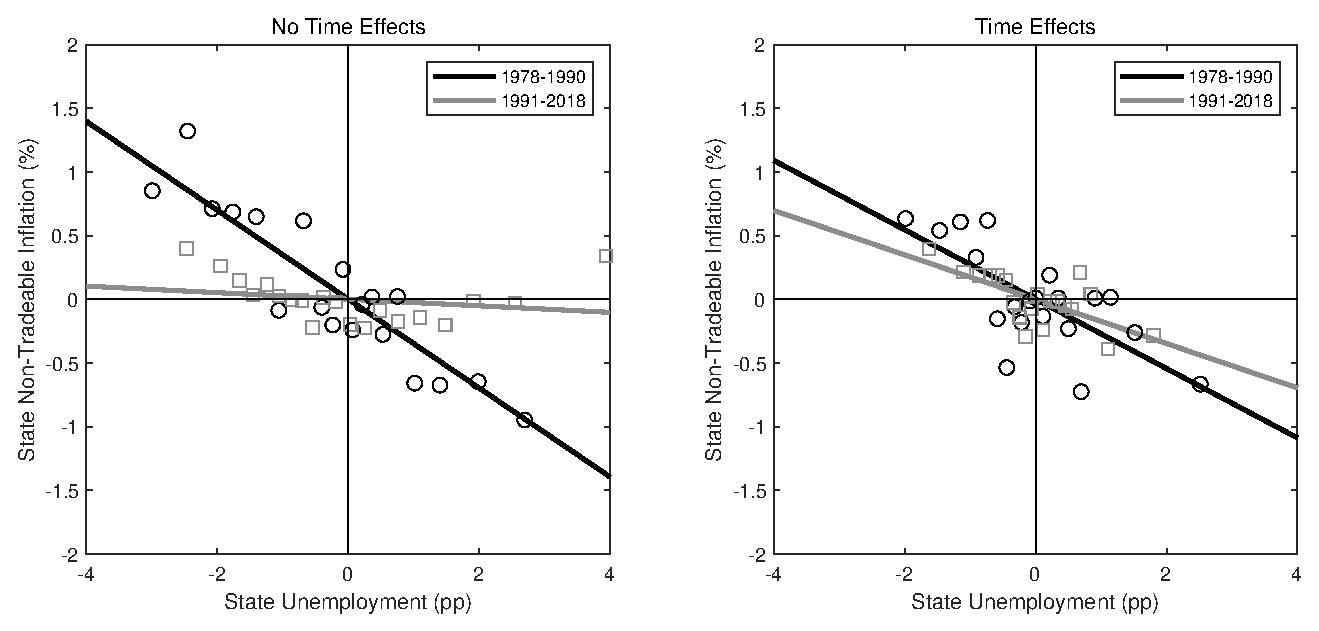
\includegraphics[width=1.0\textwidth]{figures/Fig_binscatter.eps}
		\caption{Scatterplots---Non-Tradeable Inflation and Unemployment}
	\end{figure}
	\hyperlink{Comparison}{\beamerbutton{Our Estimates Compared to Prior Work}}
\end{frame}



\begin{frame}{Aggregate Implication}\label{agg_impl}
	\begin{itemize}
		\itemsep1em 
		\item Plot RHS and LHS of
		\[ \pi_{t} - E_{t}\pi_{t+\infty} =-\kappa \zeta \tilde{u}_{t} + \omega_t\]
		assuming no supply shocks $\omega_t = 0$
		\item Scaling factor: $\zeta = 6.16$ (s.e. 1.80)
		\[\sum_{j=0}^{T} \beta^j \tilde{u}_{t+j} = \zeta \tilde{u}_{t} + \alpha + \epsilon_{t}. \]
		\item Aggregate includes housing 
		\begin{itemize}
			\item Estimate aggregate Phillips curve for shelter
			\item Data from American Community Survey for 2001-2017
			\item $\kappa = 0.0243$ (s.e. 0.0053) \hyperlink{shelter}{\beamerbutton{Table}}
			\item About four time larger than for non-shelter
		\end{itemize}
	\end{itemize}
\end{frame}



\begin{frame}[label=flatflatter]
	\vspace{30pt}
	\begin{figure}[t]
		\centering
		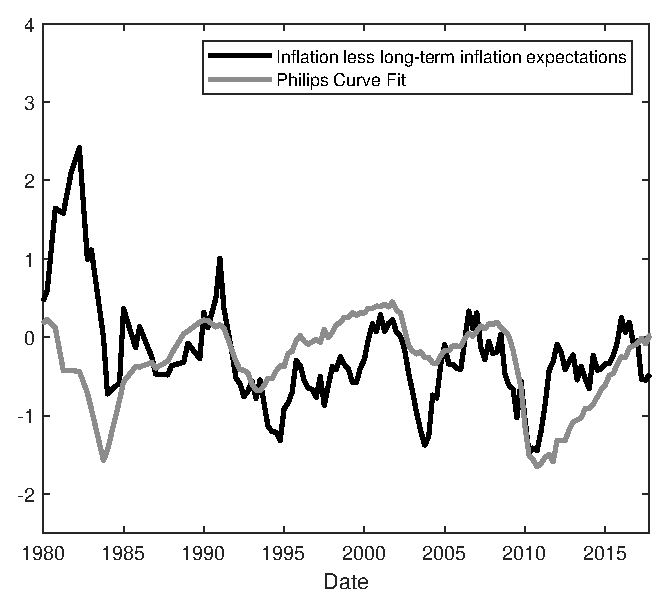
\includegraphics[width = 0.55\textwidth]{figures/fit_pc_ppt_housing.eps}
		\caption{Aggregate Phillips Curve and Housing: Predicted vs. Fit}
	\end{figure}
\end{frame}

\section{Household Wealth}

\section{Equivalence Results}

\end{document}